\documentclass{article}
\usepackage[utf8]{inputenc}
\usepackage{amsmath}
\usepackage{graphicx}
\usepackage{BeginnerStyleFile}
\graphicspath{ {images/} }

\title{Reading Summary 4.4}
\author{Evan Hughes}
\date{March 2023}

\begin{document}
\maketitle
\section*{4.4 Polynomial Functions, Roots, and Zeros}
Throughout this section $R$ is a commutative ring. Associated with each polynomial 
$a_nx^n + \cdots + a_1x + a_0$ in $R[x]$ is a function $f:R \to R$ whose rule is $f(r) = a_n r^n + \cdots + a_1 r + a_0$ for each $r \in R$.
This is called a polynomial function.

\subsection*{Example 1(from the book)}
The polynomial $x^2 + 5x + 3 \in R[x]$ induces the function $f:R \to  \mathbb{R}$ whose rule is $f(r) = r^2 + 5r + 3$ for each $r \in \mathbb{R}$.

\subsection*{Example 2}
The polynomial $x^3 + 2x + 1 \in \mathbb{Z}_3[x]$ induces the function $f:\mathbb{Z}_3 \to \mathbb{Z}_3$ whose rule is $f(r) = r^3 + 2r + 1$ for each $r \in \mathbb{Z}_3$.
Thus $f(0) = 1$, $f(1) = 0$, $f(2) = 2$

\subsection*{Definition of Roots}
Let $R$ be a commutative ring and $f(x) \in R[x]$. An element $a$ of $R$ is said to be a root of the polynomial
$f(x)$ if $f(a)=0_R$, that is, if the induced function $f:R \to R$ maps $a$ to $0_R$.

\subsection*{Theorem 4.15 The remainder theorem}
Let $F$ be a field, $f(x) \in F[x]$, and $a \in F$. The remainder when $f(x)$ is divided by the polynomial $x-a$ is $f(a)$.

\subsection*{Proof}
By the Division algorithm $f(x) = (x-a)q(x) + r(x)$ where the $r(x)$ either is 
$0_f$ or has smaller degree than the divisor $x-a$. Thus degree $r(x) = 0$ or $r(x) = 0_f$, 
In either case, $r(x) = c$ for some $c \in F$. Hence, $f(x) = (x-a)q(x) + c$ so that $f(a) = (a-a)q(a) + c = 0_f + c = c$.

\subsection*{Theorem 4.16 The Factor Theorem}
Let $F$ be a field, $f(x) \in F[x]$, and $a \in F$. Then $a$ is a root of the
polynomial $f(x)$ if and only if $x - a$ is a factor of $f(x)$.

\subsection*{Proof}
First assume that a is a root of $f(x)$. Then we have
\begin{itemize}
    \item $f(x) = (x-a)q(x) + r(x)$ 
    \item $f(x) = (x-a)q(x) + f(a)$
    \item $f(x) = (x-a)q(x)$
\end{itemize}

Therefore, $x-a$ is a factor of $f(x)$. Conversely, assume $x-a$ is a factor of $f(x)$,
say $f(x) = (x-a)g(x)$. Then $a$ is a root of $f(x)$ because $f(a) = (a-a)g(a) = 0_f g(x)$.


\subsection*{Corollary 4.18}
Let $F$ be a field, $f(x) \in F[x]$, and deg $f(x) \geq 2$. If $f(x)$ is irreducible in $F[x]$
then $f(x)$ has no roots in $F$.

\subsection*{Proof}
If $f(x)$ is irreducible, then it has no factor in the form $x-a$ in $F[x]$. Therefore it has no roots.

\subsection*{Corollary 4.20}
Let $F$ be an infinite field and $f(x), g(x) \in F[x]$. Then $f(x)$ and $g(x)$ induce the same function from $F$ to $F$ if and only if $f(x) = g(x)$ in $F[x]$.

\subsection*{Proof}
Suppose that $f(x)$ and $g(x)$ induce the same function from $F$ to $F$. Then $f(a) = g(a)$ so that $f(a) - g(a) = 0_F$. this
means that every element of $F$ is a root of the polynomial $f(x) - g(x)$. Since $F$
is infinite, this is impossible by Corollary 4.17 unless $f(x) - g(x)$ is the zero polynomial, that is, $f(x) = g(x)$.


\begin{figure}
    \centering
    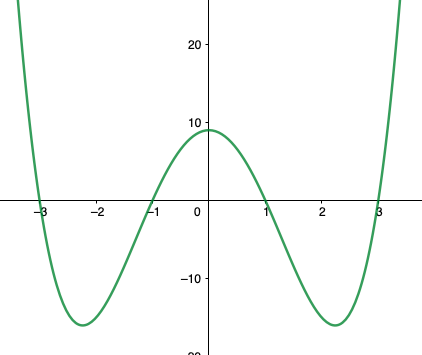
\includegraphics[width=0.6\textwidth]{zeros.png}
    \caption{Zeros in polynomials}
    \label{fig:Zeros}
\end{figure}


\end{document}